\section{Cambio de variable en integrales múltiples}

En una integral de una variable, una sustitución modifica tanto la función que se integra como el intervalo y el elemento de longitud. Si $x=g(u)$, donde $g$ es de clase $C^1$ y estrictamente creciente en $[\alpha,\beta]$, con $g(\alpha)=a$ y $g(\beta)=b$, entonces, para $f$ continua,
\[
\int_a^b f(x)\,dx=\int_\alpha^\beta f(g(u))g'(u)\,du.
\]
El factor $g'(u)$ aparece porque un incremento pequeño $\Delta u$ produce un incremento $\Delta x\approx g'(u)\Delta u$. Por ejemplo, con $x=u^2$ y $1\leq u\leq2$,
\[
\int_1^4\sqrt{x}\,dx
=\int_1^2 u(2u)\,du
=\frac{14}{3}.
\]
Se transformaron la función, $\sqrt{x}=u$, los extremos, $x=1,4$, y el diferencial, $dx=2u\,du$.

Si $g$ es estrictamente decreciente, los extremos se recorren en sentido contrario. Al describir ambos intervalos con sus extremos en orden creciente y considerar longitud sin orientación, la fórmula es
\[
\int_a^b f(x)\,dx=\int_\alpha^\beta f(g(u))|g'(u)|\,du,
\qquad g([\alpha,\beta])=[a,b].
\]
En varias dimensiones se necesita un factor semejante: mide cómo una transformación cambia áreas o volúmenes pequeños. No basta con sustituir las variables dentro de la función.

\subsection{Transformación de una región}

\begin{mydefinition}{Transformación de una región plana}
Una transformación $T$ del plano de parámetros $uv$ al plano $xy$ es una función
\[
T(u,v)=(x(u,v),y(u,v)).
\]
Si $S$ es una región del plano $uv$, su imagen es
\[
R=T(S)=\{(x(u,v),y(u,v)):(u,v)\in S\}.
\]
La transformación es inyectiva en $S$ si dos puntos distintos de $S$ tienen imágenes distintas. En ese caso, cada punto de $R$ tiene una sola representación mediante los parámetros de $S$.
\end{mydefinition}

Cambiar de variables consiste en describir los puntos de la región original $R$ mediante los puntos de otra región $S$. Las rectas $u=c$ y $v=k$ se convierten en curvas parametrizadas: con $u=c$ fijo se obtiene $v\mapsto T(c,v)$, y con $v=k$ fijo se obtiene $u\mapsto T(u,k)$. Una cuadrícula rectangular en los parámetros puede convertirse en una red de curvas en la región original.

Por ejemplo, para
\[
x=u+v,\qquad y=u-v,
\]
se tiene $x+y=2u$ y $x-y=2v$. Por tanto, los lados del cuadrado $S=[0,1]\times[0,1]$ se transforman en los segmentos de las rectas
\[
x+y=0,\quad x+y=2,\quad x-y=0,\quad x-y=2.
\]
Su imagen es el paralelogramo con vértices $(0,0)$, $(1,1)$, $(2,0)$ y $(1,-1)$. Las fórmulas inversas
\[
u=\frac{x+y}{2},\qquad v=\frac{x-y}{2}
\]
permiten verificar tanto la inyectividad como la correspondencia de las regiones. Este cambio se desarrolla en el primer ejemplo.

En general, cuando se conocen las variables nuevas $u=p(x,y)$ y $v=q(x,y)$, se sustituyen las ecuaciones de las fronteras y las desigualdades que describen $R$ para determinar $S$. Después se resuelve para $x$ e $y$, seleccionando la rama que corresponde a la región. La verificación de $T(S)=R$ evita incluir puntos ajenos o dejar partes sin cubrir.

\subsection{El factor local de cambio de área}

Se considera una transformación general $T(u,v)=(x(u,v),y(u,v))$, cuyas componentes tienen derivadas parciales continuas. Para estudiar cómo cambia el área cerca de $(u_0,v_0)$, se toma una celda rectangular
\[
S_0=[u_0,u_0+\Delta u]\times[v_0,v_0+\Delta v],
\qquad \Delta u,\Delta v>0.
\]
Se supone que $T$ es inyectiva en un entorno de esta celda. Su imagen $R_0=T(S_0)$ tiene, en general, cuatro bordes curvos. La celda es una parte pequeña de la región de parámetros; la región completa puede tener otra forma.

La función vectorial
\[
\mathbf{r}(u,v)=\langle x(u,v),y(u,v)\rangle
\]
da el vector de posición de cada punto imagen. El lado inferior de $S_0$, donde $v=v_0$, se transforma en la curva $u\mapsto\mathbf{r}(u,v_0)$; el lado izquierdo, donde $u=u_0$, se transforma en $v\mapsto\mathbf{r}(u_0,v)$. Ambas parten del punto $P=T(u_0,v_0)=(x_0,y_0)$. Los otros dos bordes se obtienen fijando $v=v_0+\Delta v$ y $u=u_0+\Delta u$.

\begingroup
\shorthandoff{>}
\begin{center}
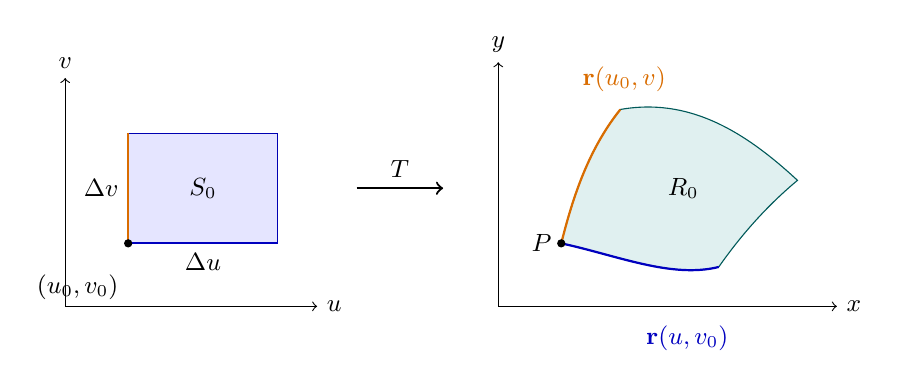
\begin{tikzpicture}[every node/.style={font=\small}]
    \draw[->] (0,0) -- (3.2,0) node[right] {$u$};
    \draw[->] (0,0) -- (0,2.9) node[above] {$v$};
    \filldraw[fill=blue!10,draw=blue!70!black] (.8,.8) rectangle (2.7,2.2);
    \draw[blue!75!black,thick] (.8,.8) -- (2.7,.8);
    \draw[orange!85!black,thick] (.8,.8) -- (.8,2.2);
    \node[below] at (1.75,.8) {$\Delta u$};
    \node[left] at (.8,1.5) {$\Delta v$};
    \fill (.8,.8) circle (1.5pt) node[below left,yshift=-8pt] {$(u_0,v_0)$};
    \node at (1.75,1.5) {$S_0$};
    \draw[->,thick] (3.7,1.5) -- (4.8,1.5) node[midway,above] {$T$};
    \begin{scope}[xshift=5.5cm]
        \draw[->] (0,0) -- (4.3,0) node[right] {$x$};
        \draw[->] (0,0) -- (0,3.1) node[above] {$y$};
        \filldraw[fill=teal!12,draw=teal!70!black]
            (.8,.8) .. controls (1.5,.65) and (2.2,.35) .. (2.8,.5)
            .. controls (3.15,1) and (3.5,1.35) .. (3.8,1.6)
            .. controls (3.1,2.25) and (2.4,2.65) .. (1.55,2.5)
            .. controls (1.15,2) and (.95,1.4) .. (.8,.8);
        \draw[blue!75!black,thick] (.8,.8) .. controls (1.5,.65) and (2.2,.35) .. (2.8,.5);
        \draw[orange!85!black,thick] (.8,.8) .. controls (.95,1.4) and (1.15,2) .. (1.55,2.5);
        \fill (.8,.8) circle (1.5pt) node[left] {$P$};
        \node at (2.35,1.5) {$R_0$};
        \node[blue!75!black,below] at (2.4,-.12) {$\mathbf{r}(u,v_0)$};
        \node[orange!85!black,above] at (1.6,2.6) {$\mathbf{r}(u_0,v)$};
    \end{scope}
\end{tikzpicture}
\end{center}
\endgroup

Los vectores tangentes a las dos curvas en $P$ son
\[
\mathbf{r}_u(u_0,v_0)=\langle x_u,y_u\rangle,
\qquad
\mathbf{r}_v(u_0,v_0)=\langle x_v,y_v\rangle,
\]
donde las derivadas del lado derecho se evalúan en $(u_0,v_0)$. Su relación con los desplazamientos entre los extremos de cada borde se obtiene de la definición de derivada. Por ejemplo,
\[
\mathbf{r}_u(u_0,v_0)
=\lim_{\Delta u\to0}
\frac{\mathbf{r}(u_0+\Delta u,v_0)-\mathbf{r}(u_0,v_0)}{\Delta u}.
\]
Por tanto, para incrementos pequeños,
\begin{align*}
\mathbf{r}(u_0+\Delta u,v_0)-\mathbf{r}(u_0,v_0)
&\approx\mathbf{r}_u(u_0,v_0)\Delta u,\\
\mathbf{r}(u_0,v_0+\Delta v)-\mathbf{r}(u_0,v_0)
&\approx\mathbf{r}_v(u_0,v_0)\Delta v.
\end{align*}
Además, la diferenciabilidad permite aproximar simultáneamente los puntos de toda la celda mediante
\[
\mathbf{r}(u_0+h,v_0+k)\approx
\mathbf{r}(u_0,v_0)+\mathbf{r}_u(u_0,v_0)h+\mathbf{r}_v(u_0,v_0)k,
\]
con $0\leq h\leq\Delta u$ y $0\leq k\leq\Delta v$. Esta expresión describe un paralelogramo que aproxima la región curva $R_0$ cerca de $P$.

\begingroup
\shorthandoff{>}
\begin{center}
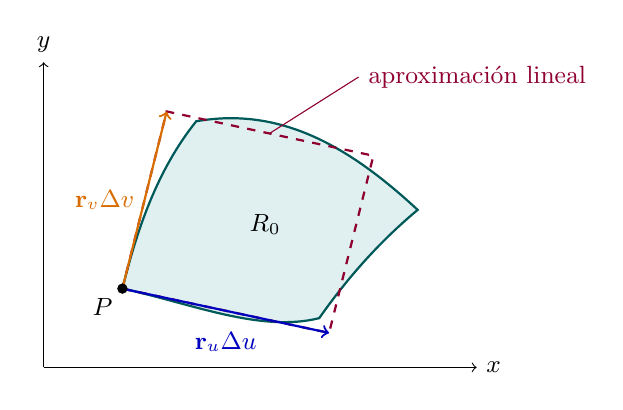
\begin{tikzpicture}[every node/.style={font=\small},scale=1.25]
    \draw[->] (0,0) -- (4.4,0) node[right] {$x$};
    \draw[->] (0,0) -- (0,3.1) node[above] {$y$};
    \filldraw[fill=teal!12,draw=teal!70!black,thick]
        (.8,.8) .. controls (1.5,.65) and (2.2,.35) .. (2.8,.5)
        .. controls (3.15,1) and (3.5,1.35) .. (3.8,1.6)
        .. controls (3.1,2.25) and (2.4,2.65) .. (1.55,2.5)
        .. controls (1.15,2) and (.95,1.4) .. (.8,.8);
    \draw[dashed,thick,purple!75!black] (.8,.8) -- (2.9,.35) -- (3.35,2.15) -- (1.25,2.6) -- cycle;
    \draw[->,thick,blue!75!black] (.8,.8) -- (2.9,.35)
        node[midway,below,yshift=-4pt] {$\mathbf{r}_u\Delta u$};
    \draw[->,thick,orange!85!black] (.8,.8) -- (1.25,2.6)
        node[midway,left] {$\mathbf{r}_v\Delta v$};
    \fill (.8,.8) circle (1.5pt) node[below left] {$P$};
    \node at (2.25,1.45) {$R_0$};
    \draw[purple!75!black] (2.3,2.38) -- (3.2,2.95)
        node[right] {aproximación lineal};
\end{tikzpicture}
\end{center}
\endgroup

La región sombreada representa la imagen curva y el contorno discontinuo representa su aproximación por los vectores tangentes. Al reducir la celda, la continuidad de las derivadas hace que la variación de esos vectores dentro de ella sea cada vez menor. Cuando $\mathbf{r}_u$ y $\mathbf{r}_v$ son linealmente independientes, el área $\Delta A$ de $R_0$ se aproxima por
\[
\Delta A\approx
\| (\mathbf{r}_u\Delta u)\times(\mathbf{r}_v\Delta v)\|
=\|\mathbf{r}_u\times\mathbf{r}_v\|\,\Delta u\,\Delta v.
\]
Para calcular este producto cruz se consideran los vectores en el espacio, con tercera componente cero:
\[
\langle x_u,y_u,0\rangle\times\langle x_v,y_v,0\rangle
=\langle0,0,x_u y_v-x_v y_u\rangle.
\]
En consecuencia,
\[
\Delta A\approx |x_u y_v-x_v y_u|\,\Delta u\,\Delta v.
\]
El factor $|x_u y_v-x_v y_u|$ describe la expansión o contracción local de área y puede variar de un punto a otro. Para una transformación de clase $C^1$ con este factor distinto de cero, el paso a elementos diferenciales da
\[
dA=|x_u y_v-x_v y_u|\,du\,dv.
\]
Así, el cálculo se aplica a regiones con bordes curvos mediante su subdivisión en celdas y la aproximación local de sus imágenes. El paralelogramo interviene como una herramienta para medir el cambio de área en cada punto. Para una transformación afín, esta aproximación coincide exactamente con la imagen de cada celda rectangular.

El valor absoluto es necesario porque un área es no negativa. El signo de la expresión sin valor absoluto distingue si la transformación conserva o invierte la orientación. Si se anula, los dos vectores tangentes son linealmente dependientes y la aproximación lineal reduce la celda a un segmento o a un punto.

\subsection{Definición de jacobiano}

\begin{mydefinition}{Jacobiano de una transformación del plano}
Para $T(u,v)=(x(u,v),y(u,v))$ de clase $C^1$, el jacobiano de $(x,y)$ respecto de $(u,v)$ es el determinante
\[
J_T(u,v)=\frac{\partial(x,y)}{\partial(u,v)}
=\begin{vmatrix}
\dfrac{\partial x}{\partial u}&\dfrac{\partial x}{\partial v}\\[4pt]
\dfrac{\partial y}{\partial u}&\dfrac{\partial y}{\partial v}
\end{vmatrix}
=x_u y_v-x_v y_u.
\]
\end{mydefinition}

El orden de las variables en el determinante importa: intercambiar dos filas o dos columnas cambia su signo, aunque no su valor absoluto.

\begin{mynote}{Cálculo del jacobiano inverso}
Supóngase que $T$ tiene una transformación inversa de clase $C^1$ y que
\[
J_T(u,v)=\frac{\partial(x,y)}{\partial(u,v)}\ne0.
\]
La regla de la cadena aplicada a $T^{-1}\circ T$ da
\[
\frac{\partial(u,v)}{\partial(x,y)}
\frac{\partial(x,y)}{\partial(u,v)}=1,
\]

En algunos casos, resulta útil expresar el jacobiano directo en términos del jacobiano inverso:
\[
\left|\frac{\partial(x,y)}{\partial(u,v)}\right|
=\frac{1}{\left|\dfrac{\partial(u,v)}{\partial(x,y)}\right|}.
\]
\end{mynote}

\subsection{Cambio de variable en una integral doble}

Realizar el cambio $T(u,v)=(x(u,v),y(u,v))$ en una integral sobre $R=T(S)$ consiste en expresar la función como $f(x(u,v),y(u,v))$, describir la región mediante $S$ y sustituir el elemento de área por $|J_T(u,v)|\,du\,dv$.

\begin{mytheorem}{Cambio de variable en el plano}
Sean $S$ y $R$ regiones compactas con fronteras formadas por un número finito de curvas de clase $C^1$ por tramos. Sea $T$ de clase $C^1$ en un abierto que contiene a $S$, tal que $T(S)=R$, $T$ lleva el interior de $S$ biyectivamente sobre el interior de $R$ y $J_T\ne0$ en el interior de $S$. Si $f$ es continua en $R$, entonces
\[
\iint_R f(x,y)\,dA
=\iint_S f(x(u,v),y(u,v))
\left|\frac{\partial(x,y)}{\partial(u,v)}\right|\,du\,dv.
\]
\end{mytheorem}

Al subdividir la región de parámetros, cada aporte se aproxima por $f(T(u,v))|J_T(u,v)|\Delta u\Delta v$. La suma de esos aportes conduce a la integral en los parámetros. El teorema garantiza la igualdad al pasar al límite.

\subsubsection{Ejemplo 1. Un paralelogramo y un cambio lineal}

Se considera
\[
I=\iint_R(x+y)\,dA,
\qquad R=\{(x,y):0\leq x+y\leq2,\ 0\leq x-y\leq2\}.
\]
Con $x=u+v$ e $y=u-v$, las desigualdades se convierten en $0\leq u\leq1$ y $0\leq v\leq1$. La inversa presentada antes verifica que el cuadrado $S$ cubre $R$ una sola vez.

\begingroup
\shorthandoff{>}
\begin{center}
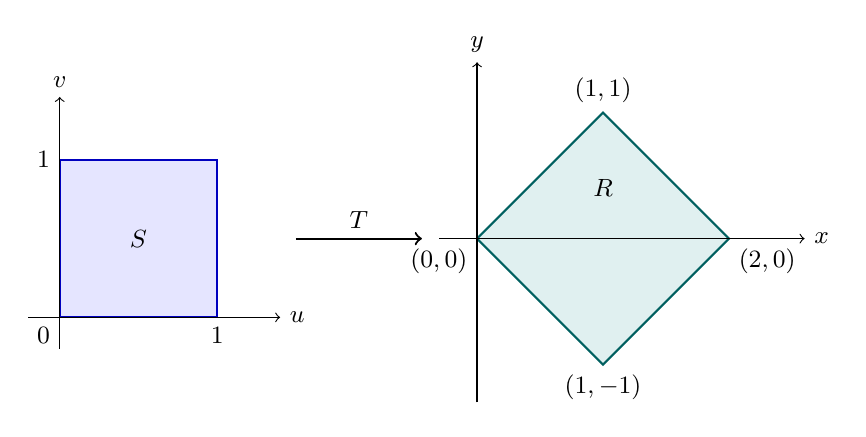
\begin{tikzpicture}[every node/.style={font=\small}]
    \begin{scope}[scale=2]
        \filldraw[fill=blue!10,draw=blue!75!black,thick] (0,0) rectangle (1,1);
        \draw[->] (-.2,0) -- (1.4,0) node[right] {$u$};
        \draw[->] (0,-.2) -- (0,1.4) node[above] {$v$};
        \node[below left] at (0,0) {$0$};
        \node[below] at (1,0) {$1$}; \node[left] at (0,1) {$1$};
        \node at (.5,.5) {$S$};
    \end{scope}
    \draw[->,thick] (3,1) -- (4.6,1) node[midway,above] {$T$};
    \begin{scope}[xshift=5.3cm,yshift=1cm,scale=1.6]
        \filldraw[fill=teal!12,draw=teal!75!black,thick] (0,0) -- (1,1) -- (2,0) -- (1,-1) -- cycle;
        \draw[->] (-.3,0) -- (2.6,0) node[right] {$x$};
        \draw[->] (0,-1.3) -- (0,1.4) node[above] {$y$};
        \node[below left] at (0,0) {$(0,0)$};
        \node[above] at (1,1) {$(1,1)$};
        \node[below right] at (2,0) {$(2,0)$};
        \node[below] at (1,-1) {$(1,-1)$};
        \node at (1,.4) {$R$};
    \end{scope}
\end{tikzpicture}
\end{center}
\endgroup

El jacobiano es constante y negativo:
\[
\frac{\partial(x,y)}{\partial(u,v)}
=\begin{vmatrix}1&1\\1&-1\end{vmatrix}=-2.
\]
Así, $dA=2\,du\,dv$ y $x+y=2u$. Se obtiene
\[
I=\int_0^1\int_0^1(2u)2\,du\,dv
=\int_0^1 2\,dv=2.
\]
Como comprobación geométrica, $R$ tiene diagonales de longitud $2$ y $2$, de modo que su área es $2$. Este valor coincide con $\iint_S2\,du\,dv$.

\subsubsection{Ejemplo 2. Fronteras hiperbólicas}

Se desea evaluar
\[
I=\iint_R\frac{x}{y}\,dA,
\qquad R=\{(x,y):x>0,\ y>0,\ 1\leq xy\leq4,\ 1\leq x/y\leq4\}.
\]
Las fronteras sugieren $u=xy$ y $v=x/y$. En el primer cuadrante se obtiene la inversa
\[
x=\sqrt{uv},\qquad y=\sqrt{u/v},
\qquad S=[1,4]\times[1,4].
\]
Las raíces positivas son necesarias para que la imagen sea precisamente $R$. Cada par $(u,v)\in S$ determina un único punto de $R$.

\begingroup
\shorthandoff{>}
\begin{center}
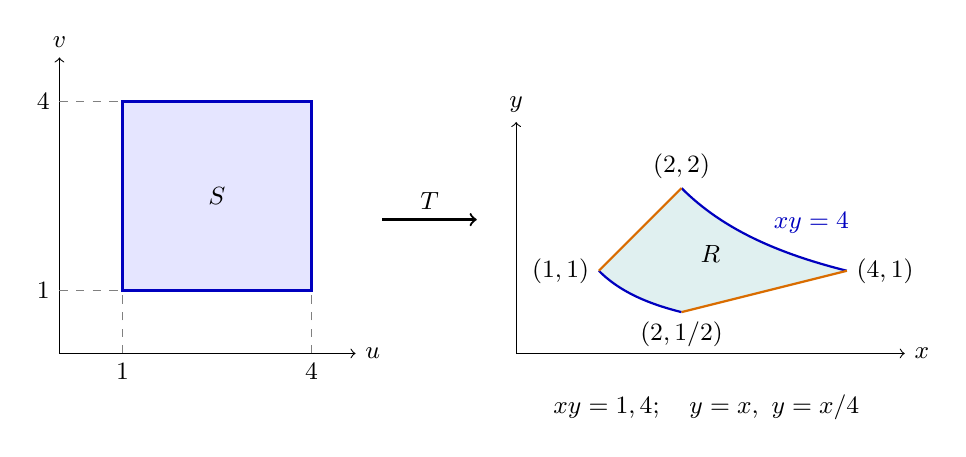
\begin{tikzpicture}[every node/.style={font=\small}]
    \begin{scope}[scale=.8]
        \filldraw[fill=blue!10,draw=blue!75!black,thick] (1,1) rectangle (4,4);
        \draw[->] (0,0) -- (4.7,0) node[right] {$u$};
        \draw[->] (0,0) -- (0,4.7) node[above] {$v$};
        \foreach \a in {1,4} {
            \draw[dashed,gray] (\a,0) -- (\a,1) (0,\a) -- (1,\a);
            \node[below] at (\a,0) {$\a$}; \node[left] at (0,\a) {$\a$};
        }
        \node at (2.5,2.5) {$S$};
    \end{scope}
    \draw[->,thick] (4.1,1.7) -- (5.3,1.7) node[midway,above] {$T$};
    \begin{scope}[xshift=5.8cm,scale=1.05]
        \fill[teal!12] plot[domain=1:2,samples=40] (\x,{1/\x}) -- (4,1)
            -- plot[domain=4:2,samples=40] (\x,{4/\x}) -- cycle;
        \draw[blue!75!black,thick] plot[domain=1:2,samples=40] (\x,{1/\x});
        \draw[blue!75!black,thick] plot[domain=2:4,samples=40] (\x,{4/\x});
        \draw[orange!85!black,thick] (1,1) -- (2,2) (2,.5) -- (4,1);
        \draw[->] (0,0) -- (4.7,0) node[right] {$x$};
        \draw[->] (0,0) -- (0,2.8) node[above] {$y$};
        \node[above] at (2,2) {$(2,2)$};
        \node[left] at (1,1) {$(1,1)$};
        \node[below] at (2,.5) {$(2,1/2)$};
        \node[right] at (4,1) {$(4,1)$};
        \node[blue!75!black,above right] at (3,1.33) {$xy=4$};
        \node at (2.35,1.2) {$R$};
        \node at (2.3,-.65) {$xy=1,4;\quad y=x,\ y=x/4$};
    \end{scope}
\end{tikzpicture}
\end{center}
\endgroup

Para evitar derivar las raíces, primero se calcula el jacobiano del cambio inverso:
\[
\frac{\partial(u,v)}{\partial(x,y)}
=\begin{vmatrix}y&x\\1/y&-x/y^2\end{vmatrix}
=-\frac{2x}{y}=-2v.
\]
Como $v\geq1$, no se anula; por reciprocidad,
\[
\frac{\partial(x,y)}{\partial(u,v)}=-\frac{1}{2v},
\qquad dA=\frac{1}{2v}\,du\,dv.
\]
La función se transforma en $x/y=v$, y resulta
\[
I=\int_1^4\int_1^4 v\frac{1}{2v}\,du\,dv
=\frac12(4-1)(4-1)=\frac92.
\]

\subsubsection{Ejemplo 3. Coordenadas adaptadas a una elipse}

Se considera la integral
\[
I=\iint_R\left(\frac{x^2}{9}+\frac{y^2}{4}\right)\,dA,
\qquad R=\left\{(x,y):\frac{x^2}{9}+\frac{y^2}{4}\leq1\right\}.
\]
El cambio
\[
x=3r\cos\theta,\qquad y=2r\sin\theta,
\qquad 0\leq r\leq1,\quad 0\leq\theta\leq2\pi,
\]
combina coordenadas polares con estiramientos en las dos direcciones. Las curvas $r=c$ son elipses y las curvas $\theta=\theta_0$ son segmentos radiales.

\begingroup
\shorthandoff{>}
\begin{center}
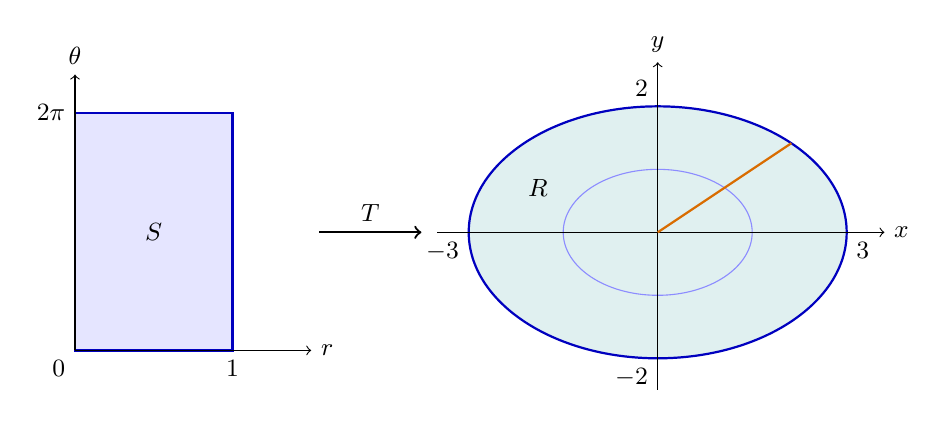
\begin{tikzpicture}[every node/.style={font=\small}]
    \begin{scope}[xscale=2,yscale=.48]
        \filldraw[fill=blue!10,draw=blue!75!black,thick] (0,0) rectangle (1,6.283);
        \draw[->] (0,0) -- (1.5,0) node[right] {$r$};
        \draw[->] (0,0) -- (0,7.3) node[above] {$\theta$};
        \node[below left] at (0,0) {$0$};
        \node[below] at (1,0) {$1$}; \node[left] at (0,6.283) {$2\pi$};
        \node at (.5,3.14) {$S$};
    \end{scope}
    \draw[->,thick] (3.1,1.5) -- (4.4,1.5) node[midway,above] {$T$};
    \begin{scope}[xshift=7.4cm,yshift=1.5cm,scale=.8]
        \fill[teal!12] (0,0) ellipse (3 and 2);
        \draw[blue!75!black,thick] (0,0) ellipse (3 and 2);
        \draw[blue!45] (0,0) ellipse (1.5 and 1);
        \draw[->] (-3.5,0) -- (3.6,0) node[right] {$x$};
        \draw[->] (0,-2.5) -- (0,2.7) node[above] {$y$};
        \draw[orange!85!black,thick] (0,0) -- ({3*cos(45)},{2*sin(45)});
        \node[below right] at (3,0) {$3$}; \node[above left] at (0,2) {$2$};
        \node[below left] at (-3,0) {$-3$}; \node[below left] at (0,-2) {$-2$};
        \node at (-1.9,.7) {$R$};
    \end{scope}
\end{tikzpicture}
\end{center}
\endgroup

Se calcula
\begin{align*}
\frac{\partial(x,y)}{\partial(r,\theta)}
&=\begin{vmatrix}3\cos\theta&-3r\sin\theta\\2\sin\theta&2r\cos\theta\end{vmatrix}\\
&=6r\cos^2\theta+6r\sin^2\theta=6r.
\end{align*}
La transformación es inyectiva para $r>0$ y $0<\theta<2\pi$. La duplicación del corte angular y la degeneración en $r=0$ afectan solamente conjuntos de área cero; la fórmula se justifica dividiendo la elipse en sectores. Como $x^2/9+y^2/4=r^2$,
\[
I=\int_0^{2\pi}\int_0^1 r^2(6r)\,dr\,d\theta
=6(2\pi)\left[\frac{r^4}{4}\right]_0^1=3\pi.
\]
El mismo cálculo con integrando $1$ da el área $6\pi$. El promedio de la función sobre la elipse es, por tanto, $1/2$.

\subsection{Extensión a integrales triples}

Una transformación espacial tiene la forma
\[
T(u,v,w)=(x(u,v,w),y(u,v,w),z(u,v,w)).
\]
Para una transformación de clase $C^1$, una caja pequeña de lados $\Delta u$, $\Delta v$ y $\Delta w$ se aproxima por un paralelepípedo con aristas
\[
\mathbf{a}\Delta u,\quad\mathbf{b}\Delta v,\quad\mathbf{c}\Delta w,
\qquad
\mathbf{a}=\langle x_u,y_u,z_u\rangle,\quad
\mathbf{b}=\langle x_v,y_v,z_v\rangle,\quad
\mathbf{c}=\langle x_w,y_w,z_w\rangle.
\]
El volumen de este paralelepípedo es el valor absoluto del producto triple escalar de sus aristas. Así,
\[
\Delta V\approx|\mathbf{a}\cdot(\mathbf{b}\times\mathbf{c})|
\,\Delta u\,\Delta v\,\Delta w.
\]

\begin{mydefinition}{Jacobiano de una transformación espacial}
El jacobiano de $(x,y,z)$ respecto de $(u,v,w)$ es
\[
J_T=\frac{\partial(x,y,z)}{\partial(u,v,w)}
=\begin{vmatrix}
x_u&x_v&x_w\\y_u&y_v&y_w\\z_u&z_v&z_w
\end{vmatrix}
=\mathbf{a}\cdot(\mathbf{b}\times\mathbf{c}).
\]
Su valor absoluto es el factor local de cambio de volumen:
\[
dV=|J_T(u,v,w)|\,du\,dv\,dw.
\]
\end{mydefinition}

\begin{mytheorem}{Cambio de variable en una integral triple}
Sean $S$ y $E$ sólidos compactos con fronteras formadas por un número finito de superficies de clase $C^1$ por tramos. Sea $T$ de clase $C^1$ en un abierto que contiene a $S$, con $T(S)=E$, que lleva el interior de $S$ biyectivamente sobre el interior de $E$ y satisface $J_T\ne0$ en el interior de $S$. Para $f$ continua en $E$,
\[
\iiint_E f(x,y,z)\,dV
=\iiint_S f(x(u,v,w),y(u,v,w),z(u,v,w))
|J_T|\,du\,dv\,dw.
\]
\end{mytheorem}

Como en el plano, se pueden dividir los sólidos en piezas y omitir fronteras de volumen cero. La transformación debe cubrir una sola vez los puntos interiores de cada pieza.

Esta fórmula recupera los factores de las coordenadas cilíndricas y esféricas. Para $x=r\cos\theta$, $y=r\sin\theta$, $z=z$,
\[
\frac{\partial(x,y,z)}{\partial(r,\theta,z)}
=\begin{vmatrix}\cos\theta&-r\sin\theta&0\\
\sin\theta&r\cos\theta&0\\0&0&1\end{vmatrix}=r.
\]
Para $x=\rho\sin\varphi\cos\theta$, $y=\rho\sin\varphi\sin\theta$ y $z=\rho\cos\varphi$, usando el orden $(\rho,\varphi,\theta)$, se tiene
\[
\frac{\partial(x,y,z)}{\partial(\rho,\varphi,\theta)}
=\begin{vmatrix}
\sin\varphi\cos\theta&\rho\cos\varphi\cos\theta&-\rho\sin\varphi\sin\theta\\
\sin\varphi\sin\theta&\rho\cos\varphi\sin\theta&\rho\sin\varphi\cos\theta\\
\cos\varphi&-\rho\sin\varphi&0
\end{vmatrix}.
\]
Al expandir por la tercera fila, el resultado es
\[
\rho^2\sin\varphi\cos^2\varphi
+\rho^2\sin^3\varphi=\rho^2\sin\varphi.
\]
En los dominios usuales $r\geq0$, $\rho\geq0$ y $0\leq\varphi\leq\pi$, ambos factores son no negativos.

\subsubsection{Ejemplo 4. Un paralelepípedo}

Se desea evaluar
\[
I=\iiint_E z\,dV,
\qquad E=\{(x,y,z):0\leq x-y\leq1,\ 0\leq y\leq1,\ 0\leq z\leq2\}.
\]
El cambio $x=u+v$, $y=v$, $z=2w$ transforma el cubo $S=[0,1]^3$ en $E$. Su inversa es $u=x-y$, $v=y$, $w=z/2$, de modo que es inyectivo.

\begingroup
\shorthandoff{>}
\begin{center}
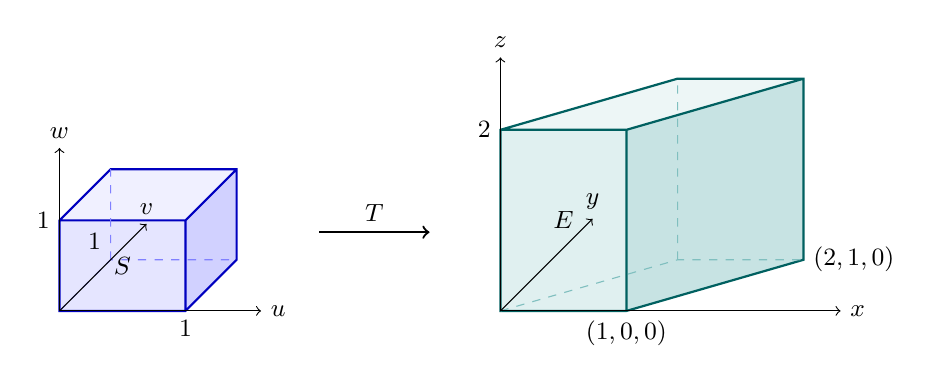
\begin{tikzpicture}[every node/.style={font=\small},
    x={(1.6cm,0cm)},y={(.65cm,.65cm)},z={(0cm,1.15cm)}]
    \begin{scope}
        \fill[blue!10] (0,0,0) -- (1,0,0) -- (1,0,1) -- (0,0,1) -- cycle;
        \fill[blue!18] (1,0,0) -- (1,1,0) -- (1,1,1) -- (1,0,1) -- cycle;
        \fill[blue!6] (0,0,1) -- (1,0,1) -- (1,1,1) -- (0,1,1) -- cycle;
        \draw[blue!75!black,thick] (0,0,0) -- (1,0,0) -- (1,1,0) -- (1,1,1) -- (0,1,1) -- (0,0,1) -- cycle
            (1,0,0) -- (1,0,1) -- (0,0,1) (1,0,1) -- (1,1,1);
        \draw[dashed,blue!50] (0,0,0) -- (0,1,0) -- (1,1,0) (0,1,0) -- (0,1,1);
        \draw[->] (0,0,0) -- (1.6,0,0) node[right] {$u$};
        \draw[->] (0,0,0) -- (0,1.7,0) node[above] {$v$};
        \draw[->] (0,0,0) -- (0,0,1.8) node[above] {$w$};
        \node[below] at (1,0,0) {$1$}; \node[left] at (0,0,1) {$1$};
        \node[above left] at (0,1,0) {$1$};
        \node at (.5,0,.5) {$S$};
    \end{scope}
    \draw[->,thick] (3.3cm,1cm) -- (4.7cm,1cm) node[midway,above] {$T$};
    \begin{scope}[xshift=5.6cm]
        \fill[teal!12] (0,0,0) -- (1,0,0) -- (1,0,2) -- (0,0,2) -- cycle;
        \fill[teal!22] (1,0,0) -- (2,1,0) -- (2,1,2) -- (1,0,2) -- cycle;
        \fill[teal!7] (0,0,2) -- (1,0,2) -- (2,1,2) -- (1,1,2) -- cycle;
        \draw[teal!75!black,thick] (0,0,0) -- (1,0,0) -- (2,1,0) -- (2,1,2) -- (1,1,2) -- (0,0,2) -- cycle
            (1,0,0) -- (1,0,2) -- (0,0,2) (1,0,2) -- (2,1,2);
        \draw[dashed,teal!50] (0,0,0) -- (1,1,0) -- (2,1,0) (1,1,0) -- (1,1,2);
        \draw[->] (0,0,0) -- (2.7,0,0) node[right] {$x$};
        \draw[->] (0,0,0) -- (0,1.8,0) node[above] {$y$};
        \draw[->] (0,0,0) -- (0,0,2.8) node[above] {$z$};
        \node[left] at (0,0,2) {$2$};
        \node[below] at (1,0,0) {$(1,0,0)$};
        \node[right] at (2,1,0) {$(2,1,0)$};
        \node at (.5,0,1) {$E$};
    \end{scope}
\end{tikzpicture}
\end{center}
\endgroup

El determinante y la integral son
\[
\frac{\partial(x,y,z)}{\partial(u,v,w)}
=\begin{vmatrix}1&1&0\\0&1&0\\0&0&2\end{vmatrix}=2,
\]
\[
I=\int_0^1\int_0^1\int_0^1 (2w)2\,dw\,dv\,du=2.
\]
El volumen de $E$ es $2$ y la altura media es $1$, lo que coincide con el valor obtenido.

\subsubsection{Ejemplo 5. Un elipsoide mediante dos transformaciones}

Se considera
\[
I=\iiint_E x^2\,dV,
\qquad E=\left\{(x,y,z):\frac{x^2}{9}+\frac{y^2}{4}+z^2\leq1\right\}.
\]
El cambio $x=3u$, $y=2v$, $z=w$ transforma la bola unitaria $B=\{u^2+v^2+w^2\leq1\}$ en $E$. Es inyectivo y su jacobiano es $3\cdot2\cdot1=6$.

\begingroup
\shorthandoff{>}
\begin{center}
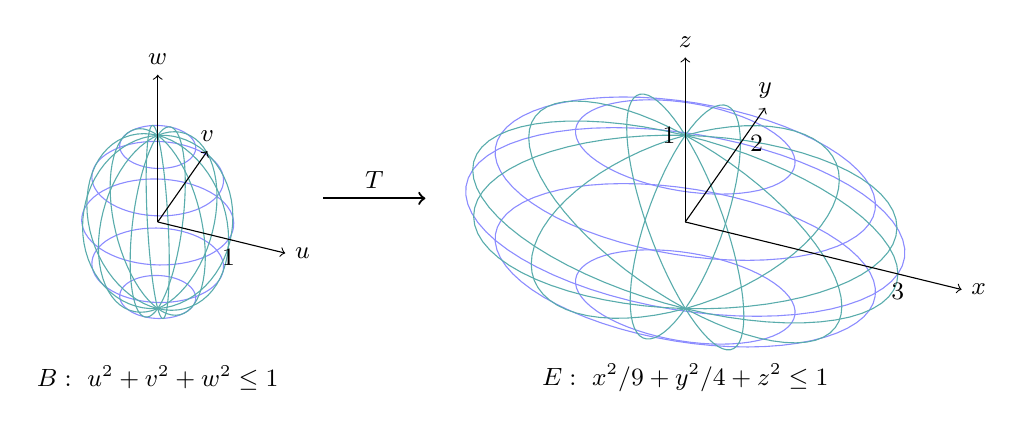
\begin{tikzpicture}[every node/.style={font=\small},
    x={(.9cm,-.22cm)},y={(.35cm,.5cm)},z={(0cm,1.1cm)}]
    \foreach \panel in {0,1} {
        \begin{scope}[xshift=\panel*6.7cm]
            \ifnum\panel=0
                \def\aa{1}\def\bb{1}
            \else
                \def\aa{3}\def\bb{2}
            \fi
            \foreach \lat in {-60,-30,0,30,60} {
                \draw[blue!45] plot[domain=0:360,samples=65]
                    ({\aa*cos(\lat)*cos(\x)},{\bb*cos(\lat)*sin(\x)},{sin(\lat)});
            }
            \foreach \ang in {0,30,...,150} {
                \draw[teal!65] plot[domain=0:360,samples=65]
                    ({\aa*cos(\x)*cos(\ang)},{\bb*cos(\x)*sin(\ang)},{sin(\x)});
            }
            \ifnum\panel=0
                \draw[->] (0,0,0) -- (1.8,0,0) node[right] {$u$};
                \draw[->] (0,0,0) -- (0,1.8,0) node[above] {$v$};
                \draw[->] (0,0,0) -- (0,0,1.7) node[above] {$w$};
                \node[below] at (1,0,0) {$1$};
                \node at (0,0,-1.8) {$B:\ u^2+v^2+w^2\leq1$};
            \else
                \draw[->] (0,0,0) -- (3.9,0,0) node[right] {$x$};
                \draw[->] (0,0,0) -- (0,2.9,0) node[above] {$y$};
                \draw[->] (0,0,0) -- (0,0,1.9) node[above] {$z$};
                \node[below] at (3,0,0) {$3$};
                \node[right] at (0,2,0) {$2$}; \node[left] at (0,0,1) {$1$};
                \node at (0,0,-1.8) {$E:\ x^2/9+y^2/4+z^2\leq1$};
            \fi
        \end{scope}
    }
    \draw[->,thick] (2.1cm,.3cm) -- (3.4cm,.3cm) node[midway,above] {$T$};
\end{tikzpicture}
\end{center}
\endgroup

Por tanto, $I=54\iiint_B u^2\,du\,dv\,dw$. Dentro de la bola se emplean coordenadas esféricas:
\[
u=\rho\sin\varphi\cos\theta,\quad
v=\rho\sin\varphi\sin\theta,\quad w=\rho\cos\varphi,
\]
con $0\leq\rho\leq1$, $0\leq\varphi\leq\pi$ y $0\leq\theta\leq2\pi$. La regla de la cadena y la multiplicación de determinantes muestran que los factores de dos cambios sucesivos se multiplican; el factor total es $6\rho^2\sin\varphi$. Se obtiene
\begin{align*}
I&=54\int_0^{2\pi}\int_0^\pi\int_0^1
\rho^4\sin^3\varphi\cos^2\theta\,d\rho\,d\varphi\,d\theta\\
&=54\left(\frac15\right)\left(\frac43\right)\pi
=\frac{72\pi}{5}.
\end{align*}

Las gráficas muestran las fronteras de los sólidos; las integrales abarcan también sus interiores.

\subsection{Ejercicios}
\begin{enumerate}
    \item Determine la imagen del cuadrado $0\leq u\leq1$, $0\leq v\leq1$ bajo $T(u,v)=(2u+v,v)$. Grafique ambas regiones y calcule $\partial(x,y)/\partial(u,v)$.

    \item Evalúe $\iint_R(x-y)\,dA$, donde $R$ está delimitada por $x+y=0$, $x+y=4$, $x-y=1$ y $x-y=3$, mediante $u=x+y$ y $v=x-y$.

    \item Evalúe $\iint_R xy\,dA$, donde $R$ es la región del primer cuadrante definida por $1\leq xy\leq3$ y $1\leq x/y\leq2$. Determine también el área de $R$.

    \item Evalúe $\iiint_E z\,dV$, donde $E$ está definido por $0\leq x-y\leq2$, $0\leq y\leq1$ y $0\leq z-x\leq1$, mediante $u=x-y$, $v=y$ y $w=z-x$.

    \item Determine $\iiint_E(x^2+y^2+z^2)\,dV$ para el elipsoide $E=\{x^2/a^2+y^2/b^2+z^2/c^2\leq1\}$, donde $a,b,c>0$.

    \item Calcule el jacobiano de la transformación $x=u^2-v^2$, $y=2uv$. Determine los puntos del plano $uv$ en los que el jacobiano se anula.

    \item Evalúe $\iint_R 1\,dA$, donde
\[
R=\left\{(x,y):\frac{x^2}{16}+\frac{y^2}{9}\leq1\right\},
\]
mediante $x=4u$ y $y=3v$.

    \item Evalúe $\iint_R(x+y)\,dA$, donde $R$ está delimitada por las rectas
\[
x+y=1,\qquad x+y=3,\qquad x-y=0,\qquad x-y=2,
\]
mediante $u=x+y$ y $v=x-y$.

    \item Evalúe $\iint_R \dfrac{1}{xy}\,dA$, donde $R$ es la región del primer cuadrante definida por
\[
1\leq xy\leq e^2,\qquad 1\leq \frac{x}{y}\leq e.
\]
Utilice $u=xy$ y $v=x/y$.

    \item Evalúe $\iint_R (x^2+y^2)\,dA$, donde
\[
R=\{(x,y):1\leq x^2+y^2\leq4,\ x\geq0,\ y\geq0\},
\]
mediante coordenadas polares.

    \item Determine el volumen del sólido $E$ definido por
\[
0\leq x-y\leq1,\qquad 0\leq x+y\leq2,\qquad 0\leq z\leq3,
\]
mediante $u=x-y$, $v=x+y$ y $w=z$.

    \item Evalúe $\iiint_E xyz\,dV$, donde
\[
E=\{(x,y,z):0\leq x\leq1,\ 0\leq y\leq x,\ 0\leq z\leq y\},
\]
mediante $x=u$, $y=uv$ y $z=uvw$.

    \item Evalúe $\iiint_E (x^2+y^2)\,dV$, donde $E$ está dentro del cilindro $x^2+y^2\leq4$, sobre el plano $z=0$ y bajo el paraboloide $z=4-x^2-y^2$. Utilice coordenadas cilíndricas.

    \item Determine el volumen de la región situada dentro de la esfera $x^2+y^2+z^2\leq9$ y sobre el cono $z=\sqrt{x^2+y^2}$. Utilice coordenadas esféricas.

    \item Determine el volumen del elipsoide
\[
\frac{x^2}{a^2}+\frac{y^2}{b^2}+\frac{z^2}{c^2}\leq1,
\qquad a,b,c>0,
\]
mediante la transformación $x=au$, $y=bv$, $z=cw$ y coordenadas esféricas en el espacio $uvw$.

    \item La transformación $T(u,v)=(u+v,u-v)$ lleva el cuadrado $S=[0,1]\times[0,1]$ sobre una región $R$. Calcule $\iint_R(x^2+y^2)\,dA$ mediante el cambio de variable y compruebe el resultado integrando directamente sobre $R$.

\end{enumerate}